\documentclass[11pt, a4paper]{article}

\usepackage[english]{babel}
\usepackage{sleek}
\usepackage{common}

\title{Introduction to Artificial Intelligence (INFO8006)}
\subtitle{Exercises 2 -- Games and adversarial search}
\date{\today}

\begin{document}

\maketitle

\section*{Learning outcomes}

At the end of this session you should be able to
\begin{itemize}[noitemsep]
    \item formulate search problems associated to a game with an Initial state, Player function, Actions, Transition model, Terminal test and Utility function (IPATTU);
    \item define the algorithms to perform game search (Minimax, $\alpha - \beta$ pruning, H-Minimax, Expectminimax, MCTS);
    \item apply Minimax, $\alpha - \beta$ pruning and H-Minimax in fully observable adversarial environments.
\end{itemize}

\section{21 misery game (January 2019)}

The game \enquote{21} is played as a game with any number of players who take turns increasing a counter. The counter starts at 1 and each player in turn increases the counter by 1, 2, or 3, but may not exceed 21; the player who says \enquote{21} or larger loses.

\begin{enumerate}
    \item Define the search problem associated with the 2-player version of the \enquote{21} game.
    
    \begin{solution}
        Let a state of the game be a pair $s = (v, p) \in \mathbb{Z} \times \cbk{0, 1}$, where $v$ is the current value of the counter and $p$ the player to play next.
        \begin{description}
            \item[Initial state] $s_0 = (1, 0)$.
            \item[Player function] $player(s = (v, p)) = p$.
            \item[Actions] $actions(s) = \cbk{1, 2, 3}$.
            \item[Transition model] For an action $a \in actions(s)$, $$result(s = (v, p), a) = (v + a,  p + 1 \bmod 2).$$
            \item[Terminal test] $terminal(s = (v, p))$ is true if $v \geq 21$, false otherwise.
            \item[Utility function] $utility(s) = 1$ if $p = 0$, $0$ otherwise.
        \end{description}
    \end{solution}
    
    \item For the following, consider the game of \enquote{5} (still in its 2-player version), which has the same rules has \enquote{21} except that you should not say 5 or more. Show the whole game tree.
    \item Using the Minimax algorithm, annotate your tree with the backed-up values, and use those values to choose the optimal starting move.
    \item Mark the nodes that would be pruned, \ie{} not evaluated, if $\alpha - \beta$ pruning was applied, assuming the nodes are generated in the optimal order for $\alpha - \beta$ pruning.
    
    \begin{solution}
        \begin{center}
            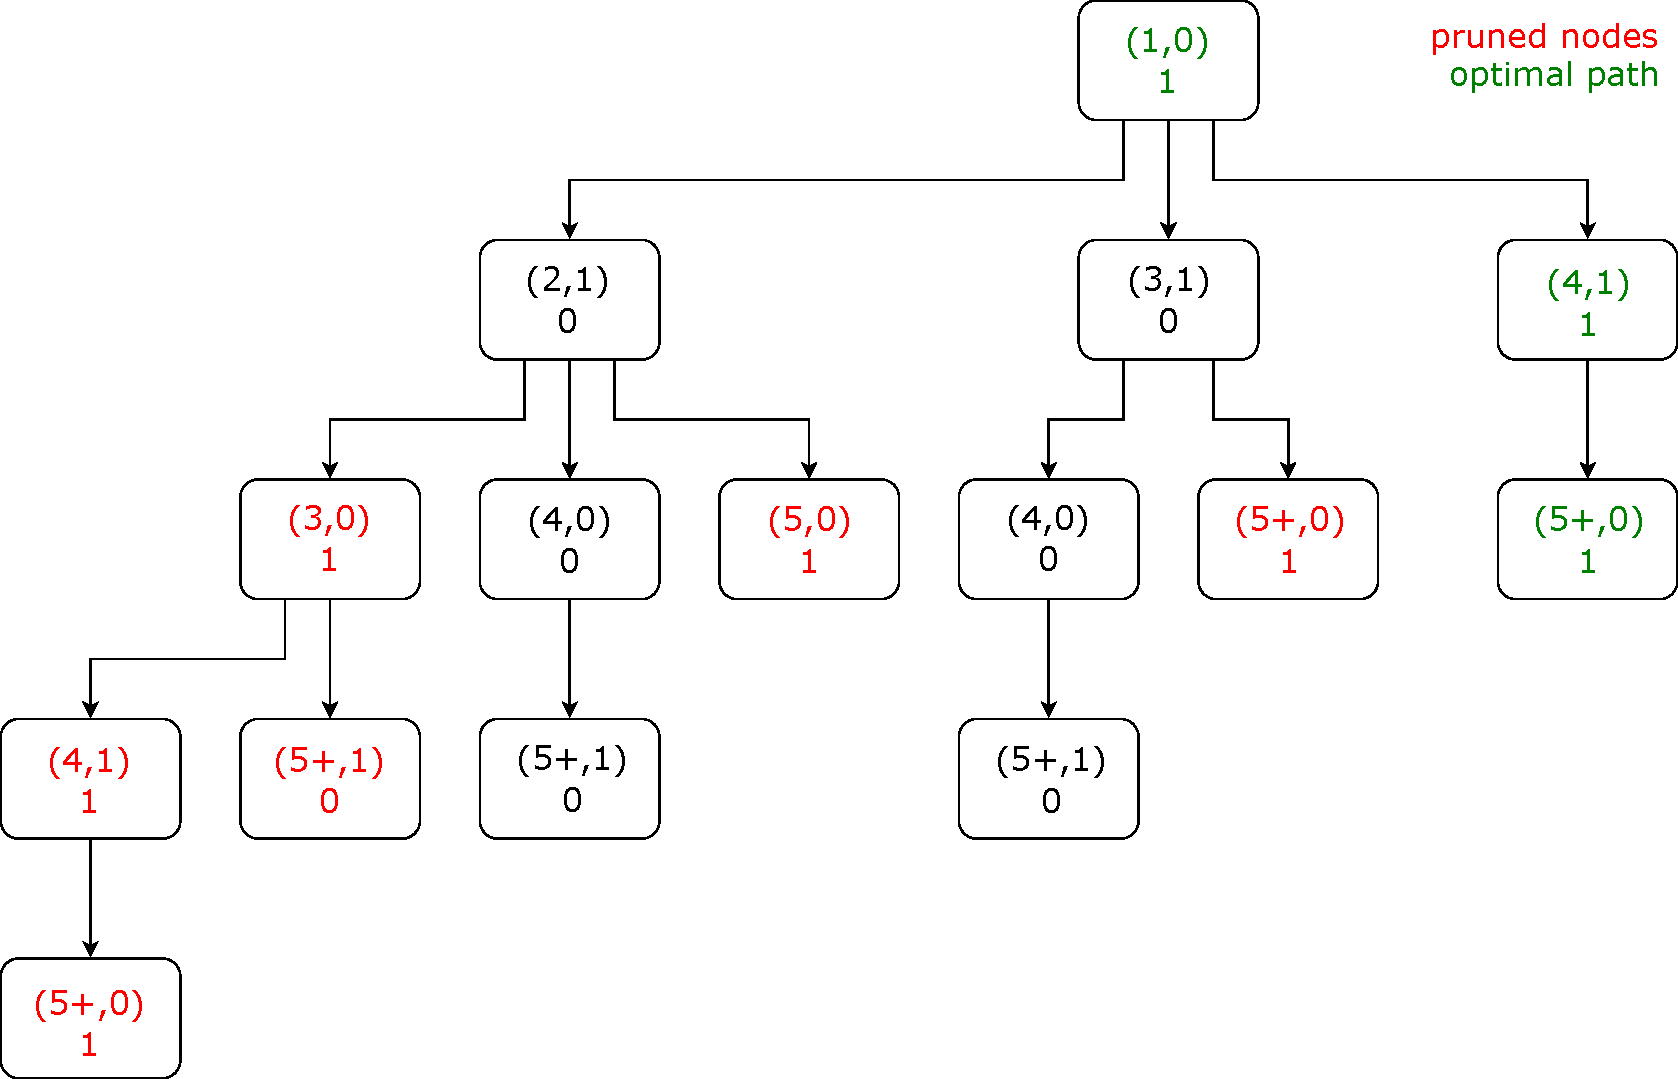
\includegraphics[width=0.9\textwidth]{figures/e2_21.pdf}
        \end{center}
    \end{solution}
\end{enumerate}

\newpage

\section{Tic-Tac-Toe (AIMA, Ex 5.9)}

Tic-Tac-Toe is a game for two players, X and O, who take turns marking the cells of a $3 \times 3$ grid. The player who succeeds in placing three of their marks in a straight line (horizontal, vertical or diagonal) wins the game. If neither of the players win before the grid is full, its a draw.

We consider X as the max player and O as the min player. We define $X_n$ as the number of rows, columns or diagonals with exactly $n$ X's and no O's. Similarly, $O_n$ is the number of rows, columns, or diagonals with just $n$ O's. A position $s$ is terminal if $X_3(s) \geq 1$, $O_3(s) \geq 1$ or if the grid is full. The utility function assigns $+1$, $-1$ or $0$ to such position, respectively. For non-terminal positions, we use an evaluation function defined as $eval(s) = 3 X_2(s) + X_1(s) - 3 O_2(s) - O_1(s)$.

\begin{enumerate}
    \item Define the search problem associated with the Tic-Tac-Toe game.
    
    \begin{solution}
        Let a state of the game be a matrix $s = (s_{ij}) \in \cbk{-1, 0, 1}^{3 \times 3}$, where the values $-1$, $0$ and $1$ respectively denote O, empty and X cells.
        \begin{description}
            \item[Initial state]
            \begin{equation*}
                s_0 = \begin{pmatrix} 0 & 0 & 0 \\ 0 & 0 & 0 \\ 0 & 0 & 0 \\ \end{pmatrix}
            \end{equation*}
            \item[Player function] The next player should be X if there are as many X's as O's on the grid and O otherwise. Choosing $+1$ for X and $-1$ for O,
            \begin{equation*}
                player(s) = \begin{cases}
                    +1 & \text{if } \sum_{i, j} s_{ij} = 0 \\
                    -1 & \text{otherwise}
                \end{cases}
            \end{equation*}
            \item[Actions] An action is represented by the position $(i, j)$ of an empty cell in the grid. Then, the set of possible actions is $actions(s) = \cbk{(i, j): s_{ij} = 0}$.
            \item[Transition model] For an action $a \in actions(s)$, $result(s, a) = s'$ is the same as $s$ except that $s'_a = player(s)$.
            \item[Terminal test] $terminal(s)$ is true if $X_3 + O_3 \geq 1$, false otherwise.
            \item[Utility function] $utility(s) = 1$ if $X_3 \geq 1$, $-1$ if $O_3 \geq 1$ and $0$ otherwise.
        \end{description}
    \end{solution}
    
    \item Approximately how many possible games states of Tic-Tac-Toe are there?
    
    \begin{solution}
        If we disregard unreachable states, we have $3^{3 \times 3} = \num{19683}$ possible states and $\fact{9} = \num{362880}$ possible games.
    \end{solution}
    
    \item Show the whole game tree starting from an empty grid down to depth 2 (one X and one O on the board), taking symmetry into account.
    \item Annotate your tree with the evaluations of all the positions at depth 2.
    \item Using the H-Minimax algorithm, annotate your tree with the backed-up values for the positions at depths 1 and 0, and use those values to choose the optimal starting move.
    \item Mark the nodes that would be pruned, \ie{} not evaluated, if $\alpha - \beta$ pruning was applied, assuming the nodes are generated in the optimal order for $\alpha - \beta$ pruning.
    
    \begin{solution}
        \begin{center}
            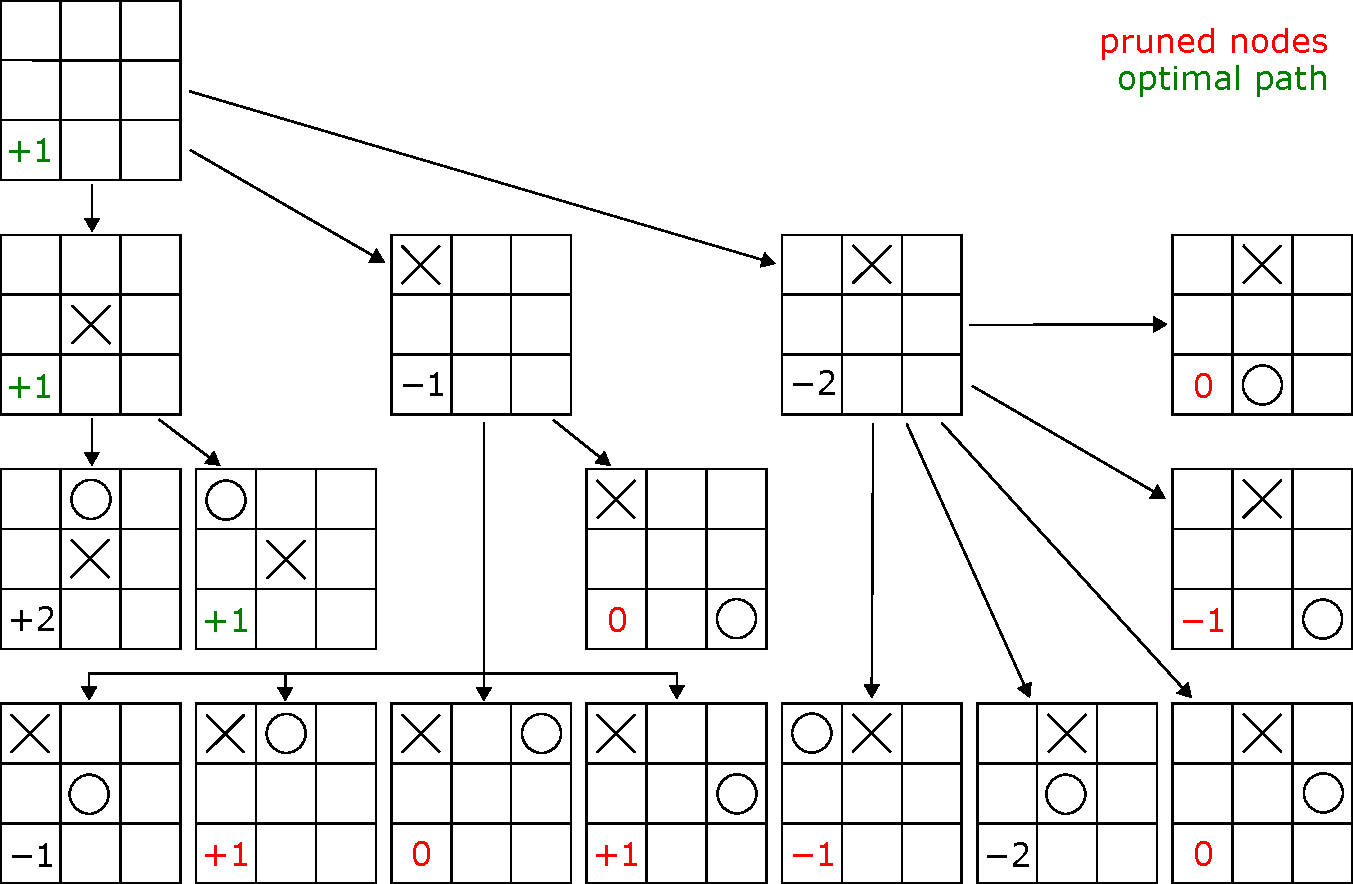
\includegraphics[width=0.8\textwidth]{figures/e2_tictactoe.pdf}
        \end{center}
    \end{solution}
    
    \item Is this evaluation function a good heuristic? If not, provide one or more states $s$ for which $eval(s)$ is misleading.
    
    \begin{solution}
        This is not a good heuristic, mainly because it does not take into account which player's turn it is. This results in states for which X is winning with lower evaluation than other states for which O is winning.
        
        \begin{center}
            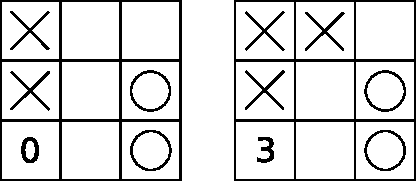
\includegraphics[width=0.3\textwidth]{figures/e2_misleading.pdf}
        \end{center}
        
        This heuristic does not preserve the Minimax \emph{ordering} of intermediate states.
    \end{solution}
    
\end{enumerate}

\newpage

\section{Quiz}

\begin{enumerate}
    \item In a fully observable, turn-taking, zero-sum game between two perfectly rational players, does it help the first player to know what strategy the second player is using, \ie{} what actions the second player will take? What if the second player is not rational ?
    
    \begin{solution}
        Since the actions taken by a perfectly rational player are always the optimal ones, the first player can already guess the moves of the second by observing the state of the game, which actually corresponds to the Minimax algorithm. Therefore, knowing the actions doesn't help.
        
        However, if the second player is not rational, it could be better to follow another strategy than Minimax, especially if the second player's strategy is known.
    \end{solution}
    
    \item What is a quiescent state?
    
    \begin{solution}
        A state in which the outcome of a game is unlikely to vary a lot in the near future. For instance, in chess, if a player has a lot more pieces than the other, the outcome of the game is likely already known, and should not change in the next few moves.
    \end{solution}
    
    \item In Monte Carlo Tree Search (MCTS), what is encouraged by each term of the sum in the formula
    \begin{equation*}
        \frac{Q(n', p)}{N(n')} + c \sqrt{\frac{2 \log N(n)}{N(n')}},
    \end{equation*}
    and what is $c$?
    
    \begin{solution}
        The first term encourages the \emph{exploitation} of states we believe to be \enquote{good}, which allows to improve our beliefs for these states. The second term encourages the \emph{exploration} of states we don't have a lot of information about. The constant $c$ controls the trade-of between exploitation and exploration.
    \end{solution}
\end{enumerate}

\newpage

\section{Chess and transposition table (AIMA, Ex 5.15)}

Suppose you have a chess program that can evaluate 16 million nodes per second.

\begin{enumerate}
    \item Decide on a compact representation of a game state for storage in a transposition table.

    \begin{solution}
        There are 32 pieces and we need to specify their positions in a $8 \times 8$ board. If a piece is not on the board anymore, we can fix its position as the position of the King. This position can be stored in \SI{6}{bits} ($2^6 = 64$), for a total of \SI{24}{o} per state.
    \end{solution}
    
    \item About how many entries can you fit in a \SI{4}{\giga o} in-memory table?
    
    \begin{solution}
        We can store roughly $\num{4e9} \times \frac{1}{24} \approx \num{160e6}$ states in the table.
    \end{solution}
    
    \item Will that be enough for the three minutes of search allocated for one move?
    
    \begin{solution}
        It is not enough to store all $\num{16e6} \times 3 \times 60 = \num{2.880e9}$ evaluated nodes.
    \end{solution}
    
    \item How many table lookups can you do in the time it would take to do one evaluation? Suppose that you have a \SI{3.2}{\giga\hertz} machine and that it takes 20 operations to do one lookup on the transposition table.
    
    \begin{solution}
        We can perform
        \begin{equation*}
            \frac{\num{3.2e9}}{\num{16e6}} \times \frac{1}{20} = 10
        \end{equation*}
        table lookups in the same amount of time as a single evaluation. This demonstrates the importance of transposition tables.
    \end{solution}
\end{enumerate}

\newpage

\section{Minimax (UC Berkeley CS188, Fall 2019)}

\begin{center}
    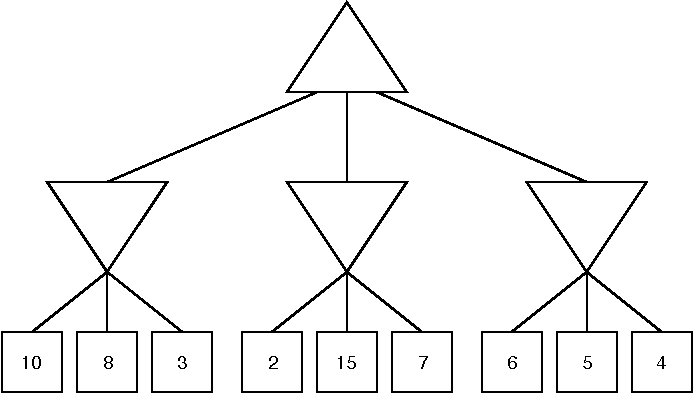
\includegraphics[width=0.6\textwidth]{figures/e2_minimax_0.pdf}
\end{center}

\begin{enumerate}
    \item Consider the zero-sum game tree shown above. Triangles that point up, such as at the top node (root), represent choices for the maximizing player; triangles that point down represent choices for the minimizing player. Assuming both players act optimally, fill in the Minimax value of each node.
    
    \begin{solution}
        \begin{center}
            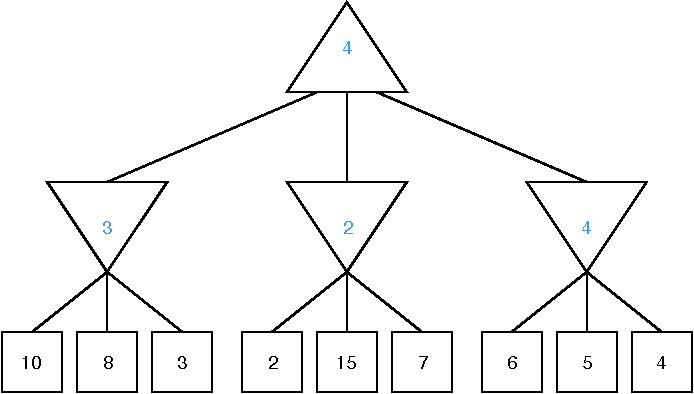
\includegraphics[width=0.6\textwidth]{figures/e2_minimax_1.pdf}
        \end{center}
    \end{solution}
    
    \item Which nodes can be pruned from the game tree above through alpha-beta pruning? If no nodes can be pruned, explain why not. Assume the search goes from left to right; when choosing which child to visit first, choose the left-most unvisited child.
    
    \begin{solution}
        \begin{center}
            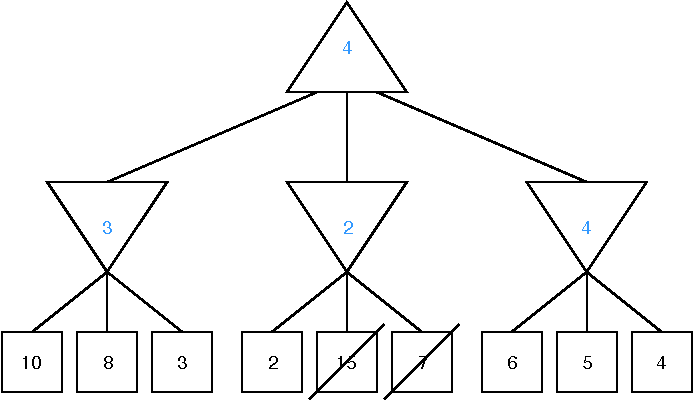
\includegraphics[width=0.6\textwidth]{figures/e2_minimax_2.pdf}
        \end{center}
    \end{solution}

    \item  Again, consider the same zero-sum game tree, except that now, instead of a minimizing player, we have a chance node that will select one of the three values uniformly at random. Fill in the Expectminimax value of each node. The game tree is redrawn below for your convenience.
    
    \begin{solution}
        \begin{center}
            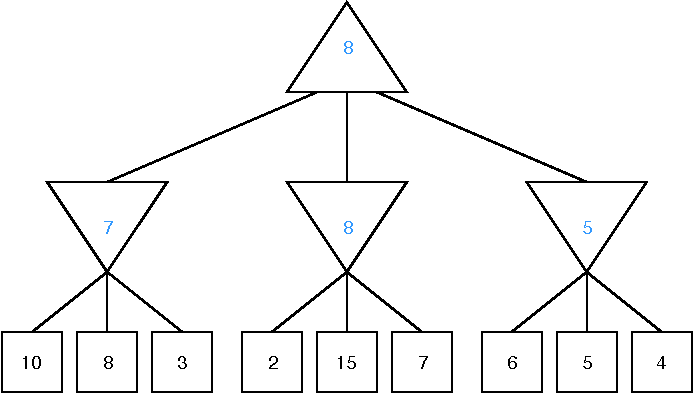
\includegraphics[width=0.6\textwidth]{figures/e2_minimax_3.pdf}
        \end{center}
    \end{solution}
    
    \item Which nodes can be pruned from the game tree above through alpha-beta pruning? If no nodes can be pruned, explain why not.
    
    \begin{solution}
        No nodes can be pruned. There will always be the possibility that an as-yet-unvisited leaf of the current parent chance node will have a very high value, which increases the overall average value for that chance node. For example, when we see that leaf 4 has a value of 2, which is much less than the value of the left chance node, 7, at this point we cannot make any assumptions about how the value of the middle chance node will ultimately be more or less in value than the left chance node. As it turns out, the leaf 5 has a value of 15, which brings the expected value of the middle chance node to 8, which is greater than the value of the left chance node.
        
        In the case where there is an upper bound to the value of a leaf node, there is a possibility of pruning: suppose that an upper bound of +10 applies only to the children of the rightmost chance node. In this case, after seeing that leaf 7 has a value of 6 and leaf 8 has a value of 5, the best possible value that the rightmost chance node can take on is $\frac{6+5+10}{3} = 7$, which is less than 8, the value of the middle chance node. Therefore, it is possible to prune leaf 9 in this case.
    \end{solution}
\end{enumerate}

\newpage

\section*{Supplementary materials}

\begin{itemize}    
    \item Chapter 5 of the reference textbook.
\end{itemize}
    
\end{document}
